%Copyright 2014 Jean-Philippe Eisenbarth
%This program is free software: you can 
%redistribute it and/or modify it under the terms of the GNU General Public 
%License as published by the Free Software Foundation, either version 3 of the 
%License, or (at your option) any later version.
%This program is distributed in the hope that it will be useful,but WITHOUT ANY 
%WARRANTY; without even the implied warranty of MERCHANTABILITY or FITNESS FOR A 
%PARTICULAR PURPOSE. See the GNU General Public License for more details.
%You should have received a copy of the GNU General Public License along with 
%this program.  If not, see <http://www.gnu.org/licenses/>.

%Based on the code of Yiannis Lazarides
%http://tex.stackexchange.com/questions/42602/software-requirements-specification-with-latex
%http://tex.stackexchange.com/users/963/yiannis-lazarides
%Also based on the template of Karl E. Wiegers
%http://www.se.rit.edu/~emad/teaching/slides/srs_template_sep14.pdf
%http://karlwiegers.com
\documentclass{scrreprt}
\usepackage{listings}
\usepackage{tabularx}
\usepackage{underscore}
\usepackage[bookmarks=true]{hyperref}
\usepackage[utf8]{inputenc}
\usepackage[portuguese]{babel}
\usepackage[inline]{enumitem}
\usepackage{hyperref}
\usepackage{placeins}
\usepackage[numberedsection]{glossaries}
\setlist[enumerate]{label=(\alph*), nosep, leftmargin=18pt, topsep=-5pt}
\hypersetup{
    bookmarks=false,    % show bookmarks bar?
    pdftitle={ESPECIFICAÇAO DE REQUERIMENTO DE  SOFTWARE},    % title
    pdfsubject={TeX and LaTeX},                        % subject of the document
    pdfkeywords={TeX, LaTeX, graphics, images}, % list of keywords
    colorlinks=true,       % false: boxed links; true: colored links
    linkcolor=blue,       % color of internal links
    citecolor=black,       % color of links to bibliography
    filecolor=black,        % color of file links
    urlcolor=purple,        % color of external links
    linktoc=page            % only page is linked
}%
\def\myversion{1.0}
\date{}

%}

\newenvironment{enumalfa}[2][label=(\alph*), nosep, leftmargin=19pt, topsep=-5pt]
{
    \begin{minipage}[t]{#2\textwidth}
    \vspace{-9pt}
    \begin{enumerate}[#1]
}
{
    \end{enumerate}
    \vspace{9pt}
    \end{minipage}
}

\newenvironment{enumalfa*}[1][label=(\alph*)]
{\begin{enumerate*}[#1]}
{\end{enumerate*}}

\newenvironment{tabela}[1]
{
    \begin{table}[!htbp]
    \def\arraystretch{1.2}
    \begin{tabular}{#1}
}
{
    \end{tabular}
    \end{table}
}

\usepackage{hyperref}
\makeglossaries

\newglossaryentry{front} {
    name=front-end,
    description={É a parte visual de um software}
}

\newglossaryentry{back} {
    name=back-end,
    description={É a parte de serviços de um software}
}


\newglossaryentry{token} {
    name=token,
    description={É uma identificação}
}

\newglossaryentry{infraAC} {
    name=infra-as-code,
    description={É uma infraestrutura definida por código}
}




\newglossaryentry{prs}{
    name=pull requests,
    description={É quando um desenvolvedor terima uma tarefa e deixa pré encaminhado para subir a alteração}
}

\newacronym{e2e}{e2e}{End-to-end é um código que testa uma funcionalidade por completo}
\begin{document}

\begin{flushright}
    \rule{16cm}{5pt}\vskip1cm
    \begin{bfseries}
        \Huge{ESPECIFICAÇÃO DE REQUERIMENTO DE SOFTWARE}\\
        \vspace{1.2cm}
        para\\
        \vspace{1.2cm}
        Gerenciador de tarefas\\
        \vspace{1.2cm}
        \LARGE{Versão \myversion}\\
        \vspace{1.2cm}
        Preparado por:  \\Lucas da Silva Santos\\Matheus Zanivan Andrade\\Rafael Nascimento Lourenço\\
        \vspace{1.2cm}
        Senac: Serviço Nacional de Aprendizagem Comercial\\
        \vspace{1.2cm}
        \today\\
    \end{bfseries}
\end{flushright}

\tableofcontents

\chapter{Casos de uso}

\vspace{1cm}

\begin{tabularx}{\textwidth}{|c|X|}
\hline
Nome do Caso de Uso & Criar usuário. \\ \hline
Ator Principal & Usuário padrão (U-001). \\ \hline
Cenário de Sucesso & Entrar no aplicativo, e se inscrever no banco de dados, ou seja, clicar no botão de registro e depois preencher os campos de e-mail e senha seguindo as restriições requeridas e finalmente clicar no botão para concluir a ação. Caso não tenha outro registro no banco de dados com o mesmo e-mail deve obter sucesso. \\ \hline
Condições Prévias & Apenas que não contenha um registro com o mesmo e-mail e siga as restrições da senha. \\ \hline
Garantia Pós-condição & Usuário inserido com sucesso no banco de dados e recebido o \gls{token} gerado automaticamente fazendo assim um login instantâneo caso ocorra sucesso. \\ \hline
Cenários Alternativos & As verificações das condições da senha serão validadas tanto no \gls{front} como no \gls{back}, pois caso ocorra algum problema por parte do usuário a parte de serviço bloqueará a ação, retornando erro. \\ \hline
\end{tabularx}

\vspace{1cm}

\begin{tabularx}{\textwidth}{|c|X|}
    \hline
    Nome do Caso de Uso & Criar organização. \\ \hline
    Ator Principal & Usuário padrão (U-001) que se tornará Dono do projeto (U-002) dentro da organização. \\ \hline
    Cenário de Sucesso & Entrar no aplicativo, e criar uma organização no banco de dados, ou seja, clicar no botão de criar organização e depois preencher os campos necessários para finalmente clicar no botão e concluir a ação. Caso não tenha outro registro no banco de dados com o mesmo nome de organização deve obter sucesso. \\ \hline
    Condições Prévias & Apenas que não contenha um registro com o mesmo nome. Esteja com um \gls{token} válido. \\ \hline
    Garantia Pós-condição & Organização criada no banco de dados e o usuário que criou se tornar Dono do projeto nesse escopo. \\ \hline
    Cenários Alternativos & Caso o usuário não esteja com um \gls{token} válido ou esteja tentando com um nome de organização já existente no banco de dados. \\ \hline
\end{tabularx}

\vspace{1cm}

\begin{tabularx}{\textwidth}{|c|X|}
    \hline
    Nome do Caso de Uso & Gerenciamento de lista de tarefas, deve ser possível criar, editar e deletar listas de tarefas. \\ \hline
    Ator Principal & Dono do projeto (U-002). \\ \hline
    Cenário de Sucesso & Entrar no aplicativo, e clicar no botão de criar lista de tarefas dentro de uma organização de acordo com as restrições desse campo. Caso o nome da lista ainda não exista na organização deve retornar sucesso. \\ \hline
    Condições Prévias & É necessário criar uma organização. Esteja com um \gls{token} válido. \\ \hline
    Garantia Pós-condição & Lista de tarefas inseridas com sucesso dentro do bando de dados. \\ \hline
    Cenários Alternativos & Caso o nome da lista de tarefas já exista dentro da organização deverá retornar erro.  \\ \hline
\end{tabularx}

\vspace{1cm}
    
\begin{tabularx}{\textwidth}{|c|X|}
    \hline
    Nome do Caso de Uso & Gerenciamento de tarefas, deve ser possível criar, editar e deletar tarefas. \\ \hline
    Ator Principal & Dono do projeto (U-002) ou Usuário padrão (U-001). \\ \hline
    Cenário de Sucesso & Entrar no aplicativo, e clicar no botão de criar tarefas dentro de uma organização e de uma lista de tarefas de acordo com as restrições desse campo. Apenas usuários atribuídos a tarefa e o Dono da organização poderão alterar o status da tarefa. \\ \hline
    Condições Prévias & É necessário criar uma organização e uma lista de tarefas e que o usuário esteja nelas. Esteja com um \gls{token} válido. \\ \hline
    Garantia Pós-condição & Tarefas inseridas com sucesso dentro do bando de dados. \\ \hline
    Cenários Alternativos & Caso de algum problema da parte de serviços retornará erro e um e-mail automático do contexto para os desenvolvedores.  \\ \hline
\end{tabularx}

\vspace{1cm}

\chapter{Diagrama de classes}

\begin{figure}[h]
    \centering
    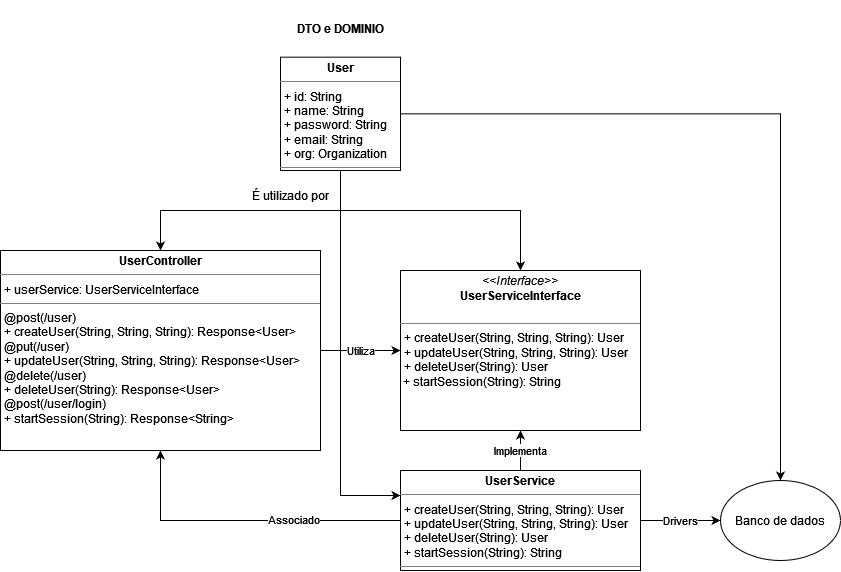
\includegraphics[width=1\textwidth]{../figures/tarefa-User.png}
    \caption{Diagrama de classe de usuário}
    \label{fig:user}
\end{figure}

\begin{figure}[h]
    \centering
    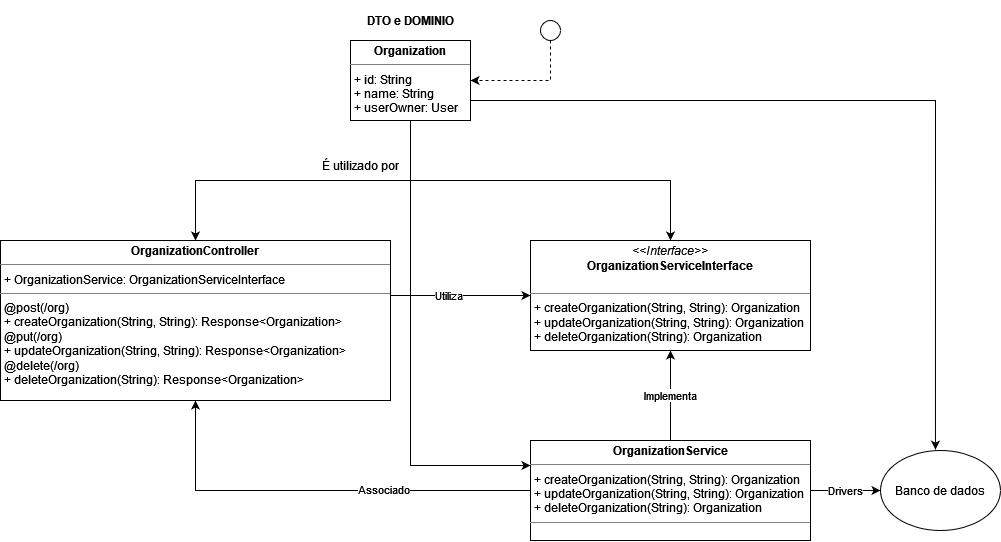
\includegraphics[width=1\textwidth]{../figures/tarefa-Org.png}
    \caption{Diagrama de classe de organização}
    \label{fig:org}
\end{figure}

\begin{figure}[h]
    \centering
    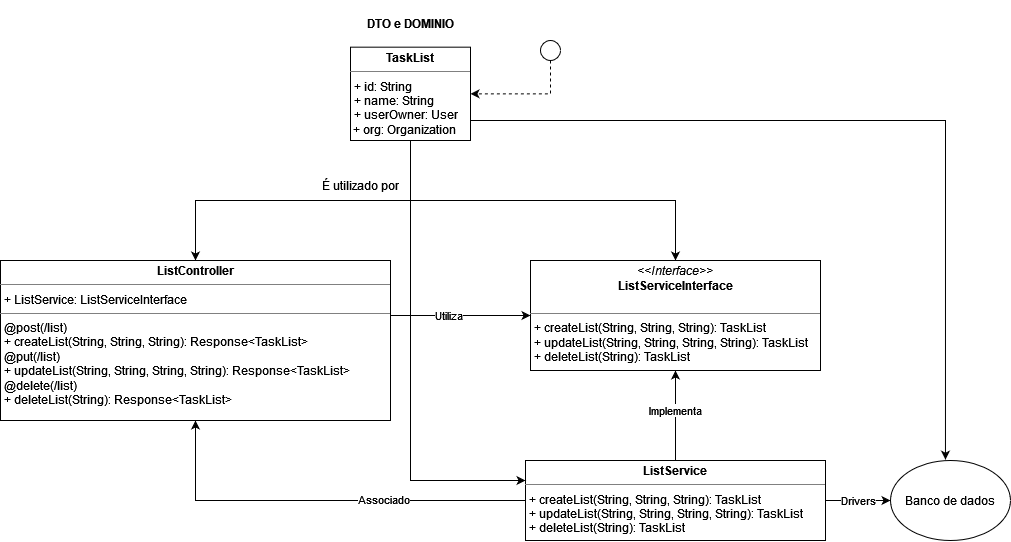
\includegraphics[width=1\textwidth]{../figures/tarefa-TaskList.png}
    \caption{Diagrama de classe de lista de tarefas}
    \label{fig:task-list}
\end{figure}

\begin{figure}[h]
    \centering
    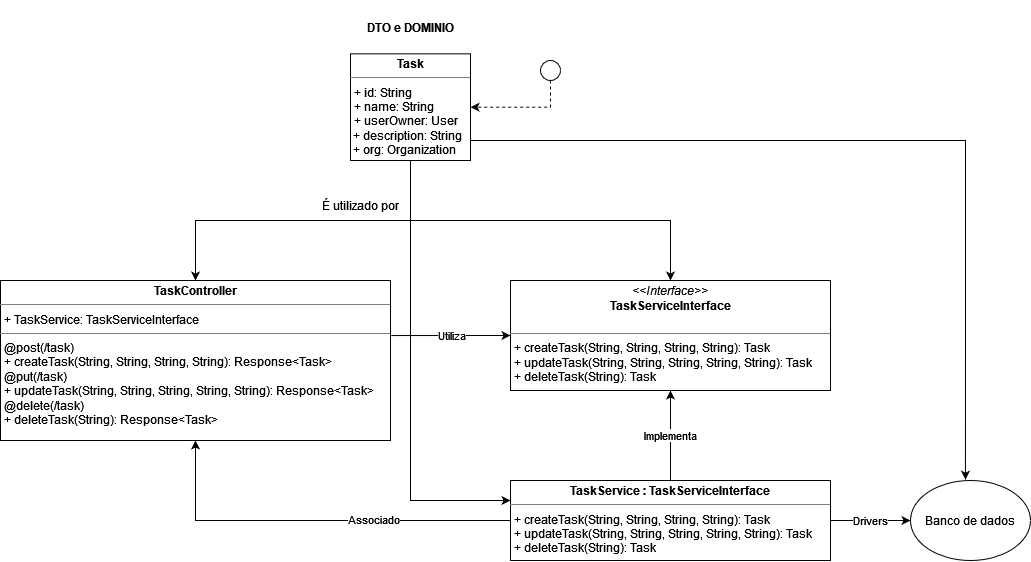
\includegraphics[width=1\textwidth]{../figures/tarefa-Task.png}
    \caption{Diagrama de classe de tarefa}
    \label{fig:task}
\end{figure}

% diagrama de sequencia

\chapter{Diagrama de sequência}

\begin{figure}[h]
    \centering
    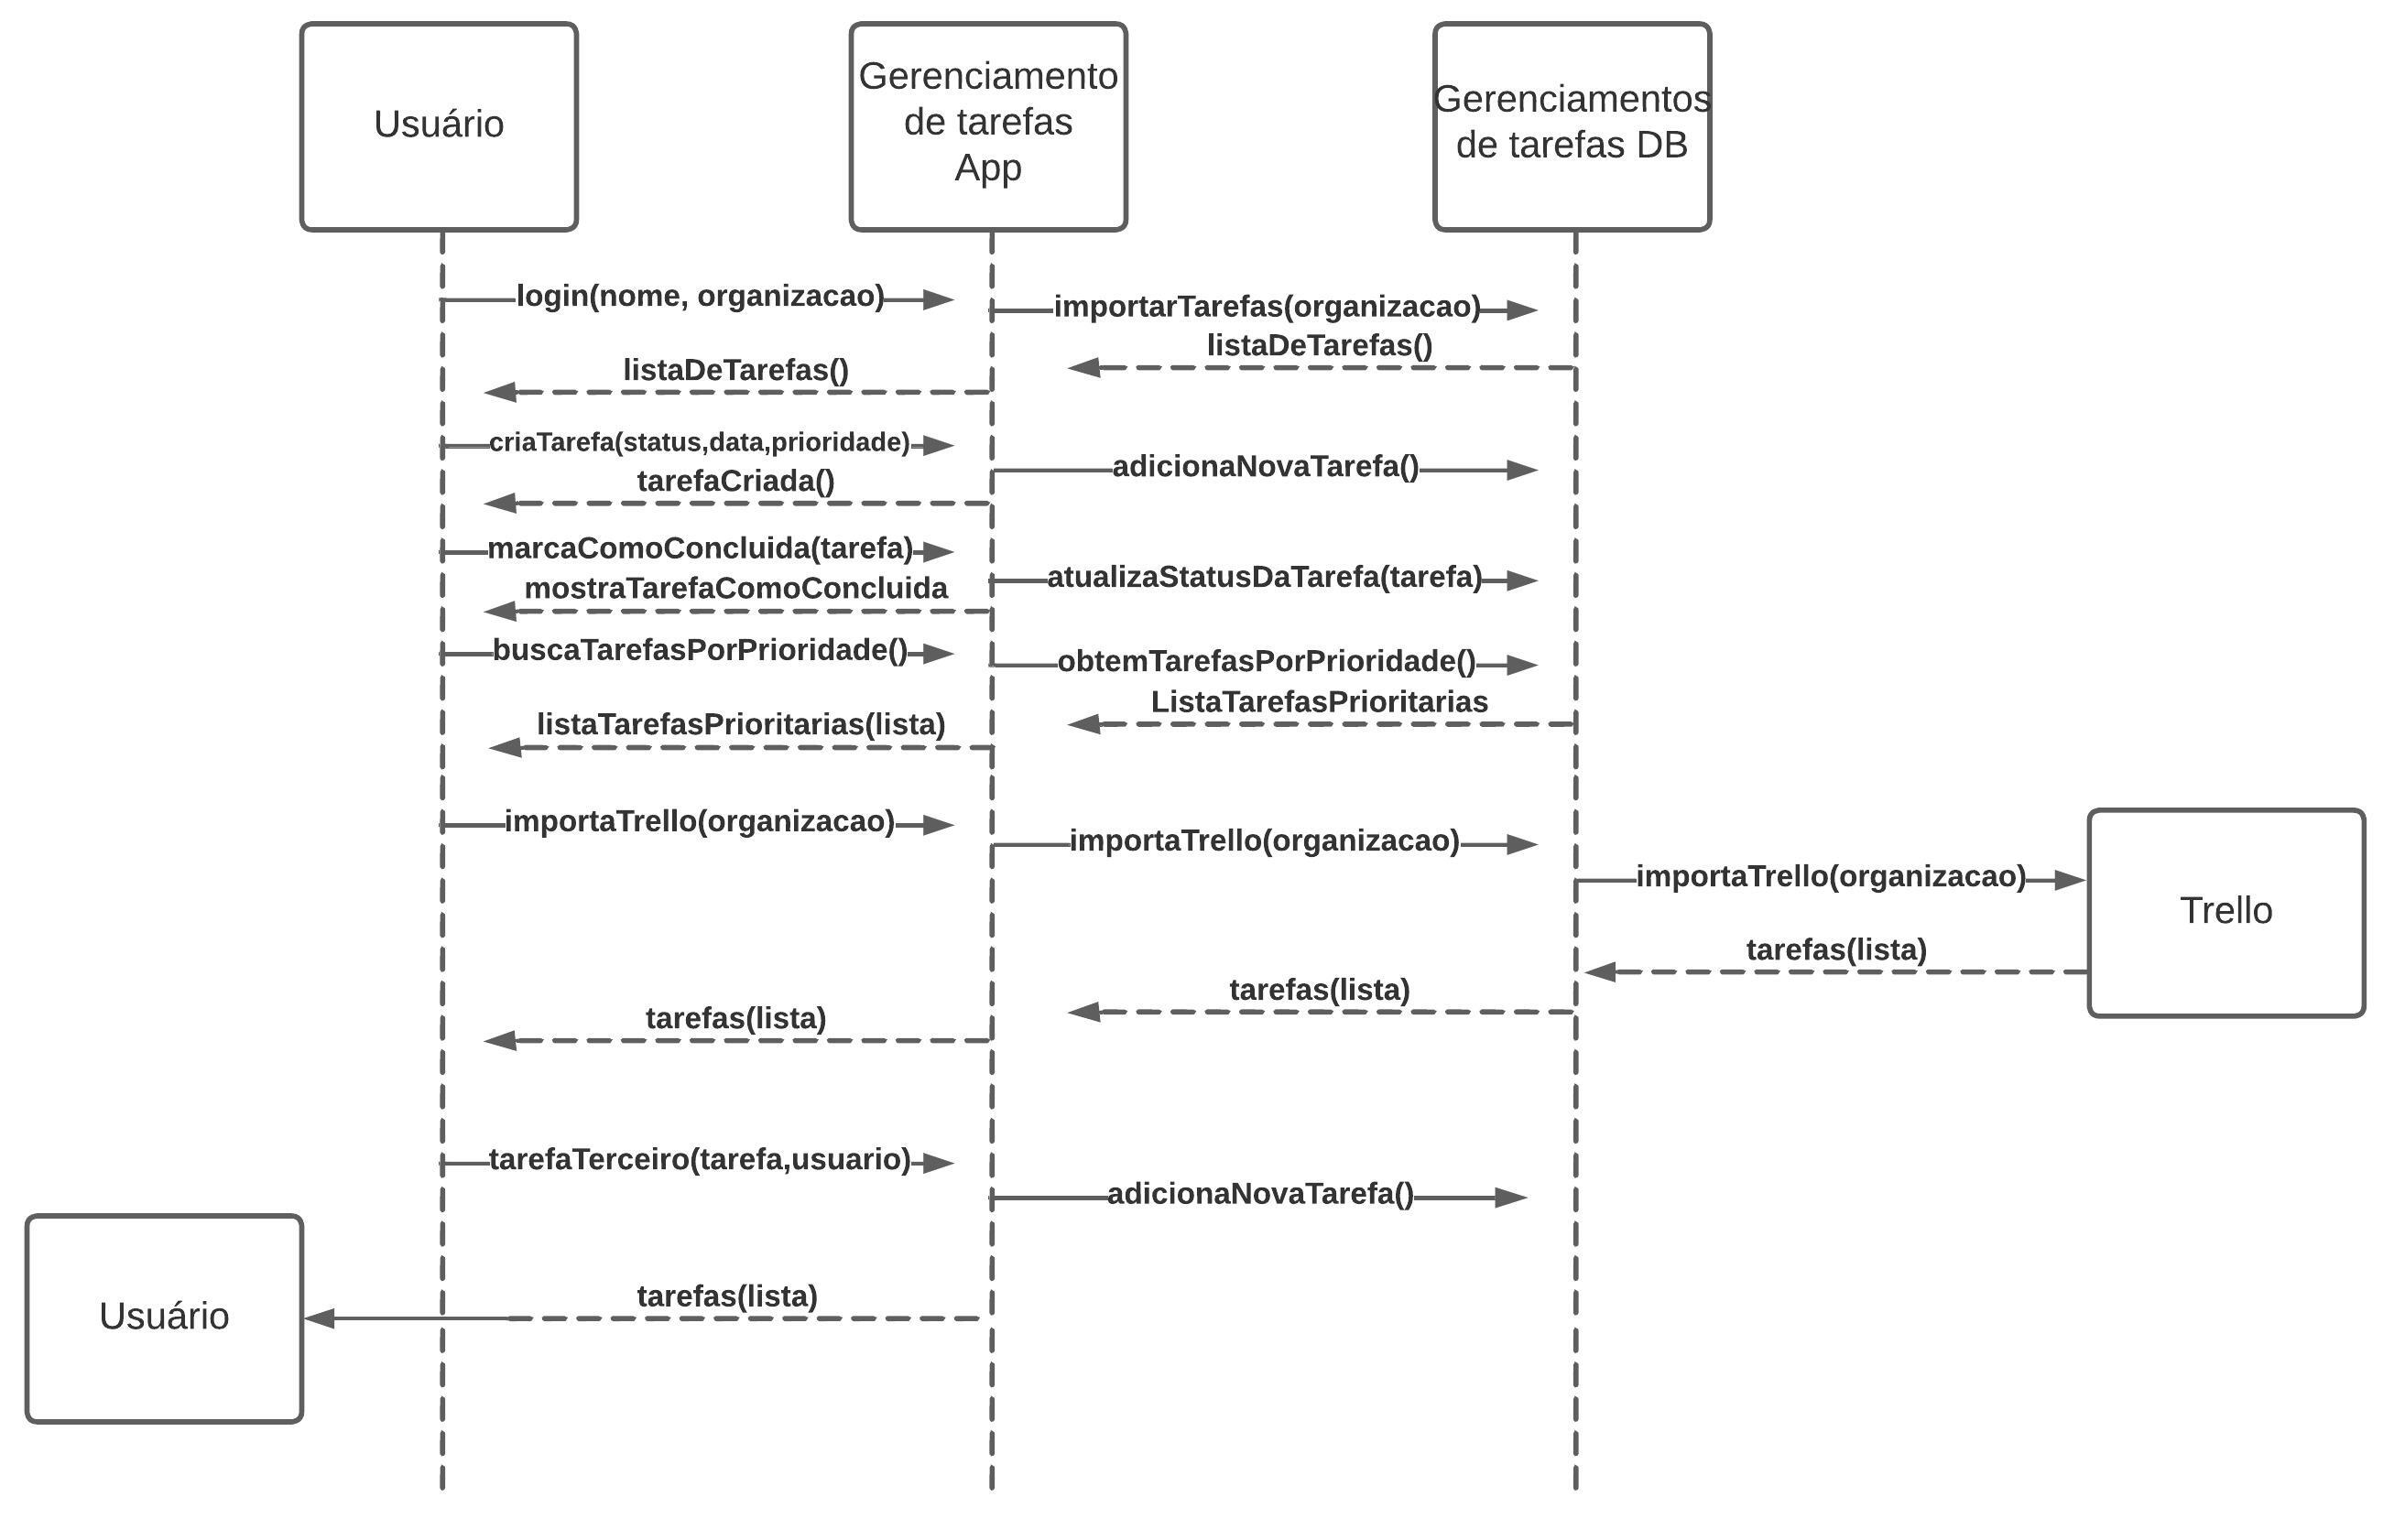
\includegraphics[width=1\textwidth]{../figures/diagramaDeSequencia.jpeg}
    \caption{Diagrama de sequência}
    \label{fig:diagramaDeSequencia}
\end{figure}


\printglossary

\end{document}